% generado por el cuaderno homónimo; no editar
\begin{subfigure}[t]{0.49\textwidth}
    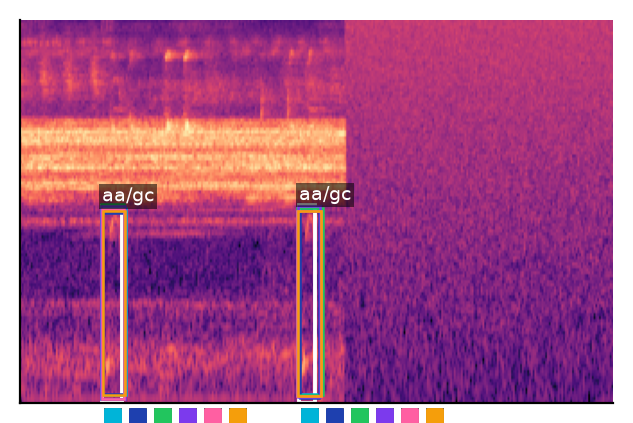
\includegraphics[width=\linewidth]{figures/RE_2-3/ventana_1}
    \caption{\code{20240608\_192212.wav}, ventana 724}
\end{subfigure}\hfill
\begin{subfigure}[t]{0.49\textwidth}
    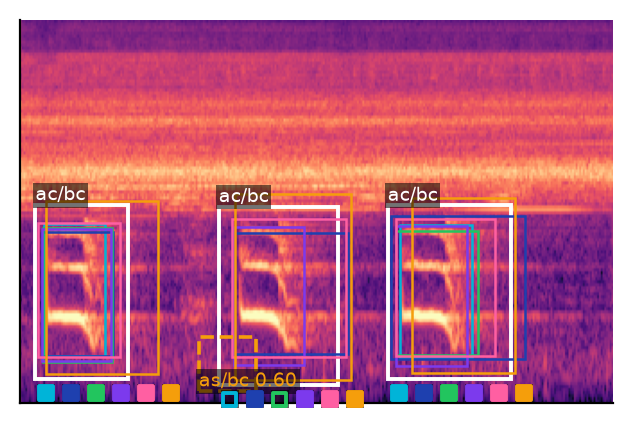
\includegraphics[width=\linewidth]{figures/RE_2-3/ventana_2}
    \caption{\code{20240913\_091420.wav}, ventana 6296}
\end{subfigure}\\[1.5ex]
\begin{subfigure}[t]{0.49\textwidth}
    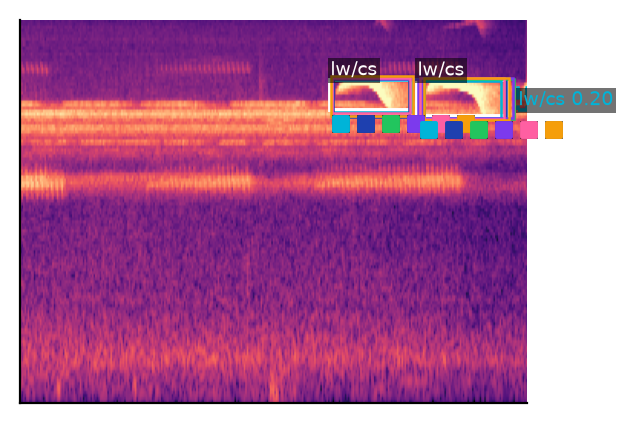
\includegraphics[width=\linewidth]{figures/RE_2-3/ventana_3}
    \caption{\code{20240621\_152146.wav}, ventana 5862}
\end{subfigure}\hfill
\begin{subfigure}[t]{0.49\textwidth}
    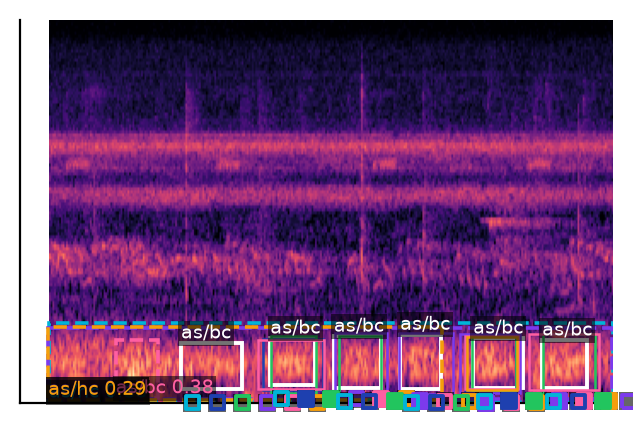
\includegraphics[width=\linewidth]{figures/RE_2-3/ventana_4}
    \caption{\code{20240604\_081131.wav}, ventana 3806}
\end{subfigure}
\par\medskip{\footnotesize \textcolor[HTML]{00B4D8}{\rule[0.4ex]{1.6em}{2.4pt}} YOLO26s @ 0,10: 6/13 acertadas, 2 FP \quad \textcolor[HTML]{1E40AF}{\rule[0.4ex]{1.6em}{2.4pt}} Faster R-CNN @ 0,74: 9/13 acertadas, 0 FP \quad \textcolor[HTML]{22C55E}{\rule[0.4ex]{1.6em}{2.4pt}} AST-DETR log-mel @ 0,27: 10/13 acertadas, 0 FP \quad \textcolor[HTML]{7C3AED}{\rule[0.4ex]{1.6em}{2.4pt}} AST-DETR aves @ 0,26: 10/13 acertadas, 1 FP \quad \textcolor[HTML]{FF5FA2}{\rule[0.4ex]{1.6em}{2.4pt}} ResNet-50 DETR @ 0,33: 10/13 acertadas, 1 FP \quad \textcolor[HTML]{F59E0B}{\rule[0.4ex]{1.6em}{2.4pt}} AST-DETR PCEN @ 0,28: 8/13 acertadas, 2 FP}
